\begin{document}
\section{Brief introduction to Neurons and Networks}
Similar to the neurons in the human brain, neurons in computer science are approaching the same concept and same ideology. 
\newline
The functionality of a neuron is to retrieve data, possibly and ideally multiple at the same time, process and output a single result. There
are many types of neurons, for introduction purposes I am just gonna mention two here.
\begin{itemize}
    \item Perceptrons
    \item Sigmoids
\end{itemize}
The more commonly used artificial neuron in Neural Network models is the Sigmoid. The reasons for that will be mentioned in the chapters
belowe.

\subsection{Percpetrons}
Perceptrons were developed in 1950 to 1960 by the scientist Frank Rosenblatt, inspired by earlier works from Waren McCulloch and Walter Pitts.
%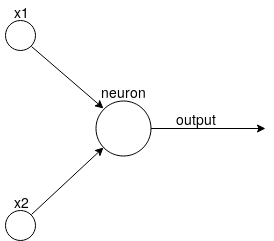
\includegraphics[width=0.5/textwidth]{images/simple_neuron.jpg}
In this example our neuron has 2 input variables and one output, in theory it can have more or less. Further more Frank Rosenblatt proposes the concept of weights for each input variable defining how important a variable is compared to another.
\newline
\begin{equation*}
    output=
    \begin{cases}
        0 \text{ if } \sum{_j}{w_jx_j \le threshold}\\
        1 \text{ if } \sum{_j}{w_jx_j > threshold}
    \end{cases}
\end{equation*}
\newpage
\noindent
A single neuron is by no means comparable to a decision making possibilities of a human being, but it can weigh variables and make decisions accordingly by defining a threshold for when a true or false gets output. Another way to create a conditional behavior is to use a bias instead of a threshold. 
%\includegraphics[width=0.5\textwidth]{images/simge_neuron_bias.jpg}
\newline
\begin{equation*}
    output=
    \begin{cases}
        0 \text{ if } \sum{_j}{w_jx_j+b \le 0}\\
        1 \text{ if } \sum{_j}{w_jx_j+b > 0}
    \end{cases}
\end{equation*}
\newline
Making it obvious that they are able to perform more complex decisions in layers.
%\includegraphics[width=0.5/textwidth]{images/neuron_network.jps}
The columns in this network are called layers, the first column is refered to as the first layers and the last one as the output one all the
ones in between are called hidden layers. 
\newline
Since the result of a perceptron can only be one or zero (true or false), one major problem someone faces when using perceptrons in more complex neural networks is that biases and weights can have weird and unwanted effects. Making perceptrons trigger where they should not, thats where sigmoids come in handy and build on top of the concept of perceptrons.

\subsection{Sigmoids}
The core principle of a sigmoid neuron is the same as the perceptrons. Just like perceptrons, sigmoids have input and output variables but
instead of just being 0 or 1 it can be anything in between 0 and 1 so 0.5234 is a valid output of a sigmoid.
%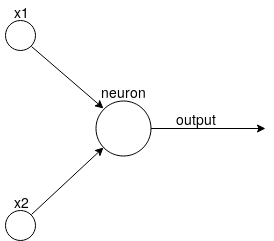
\includegraphics[width=0.5\textwidth]{images/simple_neuron.jpg}
\newline
It also has weights and biases
%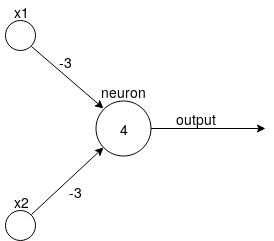
\includegraphics[width=0.5\textwidth]{images/simple_neuron_bias.jpg}
but the arithmetic function looks as follow:
is called the sigmoid function or sometimes called the logistic function.
\begin{equation*}
    \begin{split}
        \sigma(z) & = \frac{1}{1+e^{-z}}
    \end{split}
\end{equation*}
or to put it more explicit with input variables, weights and bias:
\begin{equation*}
    \begin{split}
        \frac{1}{1+exp(-\sum{_j}{w_jx_j-b})}
    \end{split}
\end{equation*}
Since the algebraic form of {$\sigma$} a is smoothed 
% smoothed graph here
And not a step function:
% step grap here
It is the only place where sigmoid differs from the perceptron.
\newpage

\section{Current state}
Object Detection in dealing with two major problems and therefore can be split into two processes, these are object localization and object classification of multiple objects in one image. There are many approaches in current Neural Network models to perform these actions.
There are models which have a multi layer architecture, each performing complex tasks such as analyzing, localizing and classifying each sections individually, making the cost high and the network in general slow but accurate.
There models that combine functionality in one layer so that one layer for instance localizes and classifies at the same time, is making the model more flexible, smaller and therefore faster but less accurate.
The trade off between accuracy and speed is something that all networks deal with nowadays especially if the goal is to have a near real life object
detection system which is still reliable and accurate when doing so.
\newline
There are multiple algorithms covering various forms of this formula, called RCNN, F-RCNN, SSD, YOLO but first we will cover the approach of
detecting interesting regions in an image because this is a key problem in object detection.

\subsection{Approaches to Object Localization}
The segmentation of an image is the key approach to Object Localization, since images are always hierarchical the segmentation as well has
to be hierarchical. It has to be able to cover different criteria and forms, where maybe objects are part of a bigger total or just single
parts inside another one. Since is not feasible to compute every possibility inside an image there has to be some kind of separation
through grids and scales.
\newline
As there are many approaches to algorithms how to analyze and classify regions, there are many approaches for algorithms to detect
interesting sections of an image which may contain objects.

\subsubsection{Exhaustive Search}
Since an object can be located anywhere in an image the scope to look for it is enormous making the computational cost for such search very
expensive. To compensate for this cost most exhaustive search approaches such as the sliding window approach, constraint the size and aspect
ratio of the window over the grid, also using weak classifiers and economic image features such as histogram of oriented gradients
(HOG).\cite{selectivesearch}
\newline
HOG approaches the problem of recognizing and detecting objects in an unkown image through detecting corners, their distribution and their
orientation. Analyzing these you are able to seperate the image in multiple partitions or detect similiar regions in different images.
Robert K. McConnell described the concept in a patent in 1986. It became known in 2005 through a publication from Navneet Dalal and Bill
Triggs.\cite{wiki_hog}
\newline
\begin{center}
    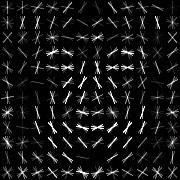
\includegraphics[width=0.5\textwidth]{images/Dlib_Learned-HOG-Detector.jpg} \cite{wiki_hog}
\end{center}

\subsubsection{Selective Search}

\subsubsection{Region Proposal Network}

\subsection{Approaches to Object Classification}

\end{document}                    
